\documentclass[a4paper,10pt]{report}

\usepackage[utf8]{inputenc}
\usepackage[frenchb]{babel}
\usepackage[T1]{fontenc}
\usepackage[top=2cm, bottom=2cm, left=2cm, right=2cm]{geometry}
\usepackage{listings}
\usepackage{hyperref}
\usepackage{color}
\usepackage{fancyhdr}
\usepackage{graphicx}
\usepackage{multicol}

\title{Rapport Technique}

\author{Florian Barrois \and Nicolas Devillers \and Valentin Jeanroy \and Mehdi Loisel \and Jean Mercadier \and Ismail Taleb \and Willeme Verdeaux}

\definecolor{dkgreen}{rgb}{0,0.6,0}
\definecolor{gray}{rgb}{0.5,0.5,0.5}
\definecolor{mauve}{rgb}{0.58,0,0.82}

\newcommand{\code}[1]{\texttt{#1}}

\lstset{frame=tb,
  language=Java,
  aboveskip=3mm,
  belowskip=3mm,
  showstringspaces=false,
  columns=flexible,
  basicstyle={\small\ttfamily},
  numbers=none,
  numberstyle=\tiny\color{gray},
  keywordstyle=\color{blue},
  commentstyle=\color{dkgreen},
  stringstyle=\color{mauve},
  breaklines=true,
  breakatwhitespace=true
  tabsize=3
}

\begin{document}
  \begin{titlepage}

    \begin{center}
    ~\\~\\~\\~\\~\\
    \Huge
    Projet STCal\\
    \LARGE
    Rapport technique\\
    ~\\~\\~\\~\\~\\~\\
      \begin{multicols}{3}
	\large
	Florian Barrois\\Mehdi Loisel\\
	\columnbreak 
	Nicolas Devilers\\Jean Mercadier\\Willeme Verdeaux\\
	\columnbreak
	Valentin Jeanroy\\Ismail Taleb
      \end{multicols}
    \end{center}


  \begin{center}
  ~\\~\\~\\~\\~\\~\\~\\~\\~\\~\\~\\~\\
  
\includegraphics{../general/iutbm.jpeg}
  ~\\~\\~\\~\\~\\
  \large
  Année 2013-2014
  \end{center}

\end{titlepage}

\thispagestyle{headings}


\tableofcontents

\chapter*{Introduction}

À travers ce manuel nous allons expliquer comment a été pensée l'application avec des détails techniques pour faciliter la reprise du travail à venir sur ce projet.

\chapter{Installation}

	\section{Installation}

		\subsection{Prérequis}

			Pour lancer l'application, il est obligatoire d'avoir a disposition un serveur MySQL. Ainsi au démarrage le programme chargera ses information dans la base de donné. Mais si celle-ci n'existe pas, elle sera créée avec le nom de stcal.

			Cette base de données permet ainsi à l'application de sauvegarder et recharger ses données au lancement et à la fin de l’exécution du programme.

			\paragraph*{note:}
			  Il est conseillé de créer un utilisateur spécifique au programme qui aura tous les privilèges sur la base de données stcal.

		\subsection{Obtenir l'application}

			L'intégralité de l'application se trouve sur GitHub sur le dépôt stcal: \href{https://github.com/Ricain/stcal}{https://github.com/Ricain/stcal}
	
			\paragraph[Binaire]{Exécutable}
			  Pour obtenir un exécutable de l'application, soit un fichier jar il suffit de le télécharger sur GitHub à l'URL suivante: \href{https://raw.githubusercontent.com/Ricain/stcal/Main/stcal.jar}{https://raw.githubusercontent.com/Ricain/stcal/Main/stcal.jar}

			\paragraph[Code source]{Code source}
			  Pour obtenir le code source d'une manière ``propre'' (sans le télécharger directement dans un fichier zip sur GitHub), il suffit de cloner le projet:

			  \code{\$ git clone https://github.com/Ricain/stcal}

			  L'intégralité du projet sera clonée dans un répertoire stcal sous le répertoire courant. Cela nécessite d'avoir git d'installé. Dans un environnement Linux, le gestionnaire de paquets permet de l'installer. 
			  Sur un mac, il faut installer et exécuter la commande suivante après avoir installé Xcode:

			  \code{\$ xcode-select --install}

			  Une fois git installé il est possible de faire des ``commit'' et des ``pull request''.

			\paragraph[IDEA]{IDEA}
			Il est cependant possible de cloner directement le projet à partir d'\href{http://www.jetbrains.com/idea/}{IntelliJ IDEA}. Pour cela il suffit d'importer un projet à partir d'un VCS (Version Control System). L'IDE vous demandera le lien GitHub de l'application énnoncé plus haut.

			\paragraph*{}
			L’environnement de développement doit être configuré de manière à ce que les fichiers \textit{jar} soient bien en inclus en tant que \textit{library}.

\chapter{Structure}

	\section{Arborescence}

	\paragraph*{}
	Ci-dessous ce trouve arborescence du projet. On y compte 6 dossiers et 52 classes.

	\begin{verbatim}
	    stcal
	    |-- Stcal.java
	    |-- control
	    |   |-- CALsettings.java
	    |   |-- CustomRenderer.java
	    |   |-- DBTools.java
	    |   |-- DBsettings.java
	    |   |-- Datas.java
	    |   |-- ListTools.java
	    |   |-- Message.java
	    |   |-- OSplitCsv.java
	    |   |-- Outics.java
	    |   |-- ScriptRunner.java
	    |   |-- Settings.java
	    |   |-- exceptions
	    |   |   |-- MaxSoutenanceException.java
	    |   |   |-- NoSuchSettingException.java
	    |   |   \-- NothingToSaveException.java
	    |   |-- parserDate.java
	    |   \-- parserPeriod.java
	    |-- don
	    |   |-- DAgenda.java
	    |   |-- DCandide.java
	    |   |-- DCouple.java
	    |   |-- DCreneau.java
	    |   |-- DEtudiant.java
	    |   |-- DListe.java
	    |   |-- DPersonne.java
	    |   |-- DProf.java
	    |   |-- DSalle.java
	    |   |-- Soutenance.java
	    |   |-- Type.java
	    |   \-- manager
	    |       |-- DCandideManager.java
	    |       |-- DCreneauManager.java
	    |       |-- DEtudiantManager.java
	    |       |-- DProfManager.java
	    |       |-- DSalleManager.java
	    |       |-- Manager.java
	    |       |-- SalleManager.java
	    |       |-- Singleton.java
	    |       \-- SoutenanceManager.java
	    \-- fen
	        |-- CreneauTableModel.java
	        |-- DCoupleTransferHandler.java
	        |-- DynamicTree.java
	        |-- DynamicTreeOperator.java
	        |-- FCal.java
	        |-- FChooser.java
	        |-- FCsv.java
	        |-- FExportIcs.java
	        |-- FInterface.java
	        |-- FLier.java
	        |-- FMenu.java
	        |-- FSalles.java
	        |-- FSettings.java
	        |-- FStage.java
	        \-- FTab.java
	\end{verbatim}



	\section{MVC}

	L'arborescence du projet a été pensée pour respecter au mieux le \textbf{m}odèle \textbf{v}ue \textbf{c}ontroleur. Sous le répertoire \textit{src} on trouve trois autres répertoires:
	\begin{description}
		\item[control] contient l’ensemble des classes moteur à l'application (contrôleur).
		\item[fen] abréviation de fenêtre, contient l’ensemble des classes permettant de dessiner l'application (vue).
		\item[don] abréviation de données, contient l’ensemble des classes concernant les données de l'application (modèle).
	\end{description}

		\subsection{Modèle}

			\paragraph*{}
			Le modèle constitue les données de l’application. L’ensemble des classes prévues à cette effet sont stockées sous le répertoire \textit{don}. On y trouve des classes comme:
			\begin{itemize}
				\item Étudiant
				\item Soutenance
				\item Prof
				\item Agenda
			\end{itemize} 

			\paragraph*{}
			Sauvegarder les données de l'application permet non seulement de garder un historique des stages mais également de ré-ouvrir l'application et de la retrouver tel qu'on l'a fermée. À cet effet on trouve un sous répertoire \textit{manager} qui contient un ensemble de classes permettant de faire le lien entre la base de données et le modèle de données de l'application. 
			Chaque manager \textbf{doit} implémente l'interface manager afin de respecter le concept de JBDD (enseigné en semestre 4).

		\paragraph*{}
		Le script qui permet d'installer la base de données se trouve dans le répertoire \textit{res} (ressources).

			\paragraph*{}
			Les classes constituant le répertoire \textit{don} on était pensées sur un modèle bien précis. On verra le MCD et l'UML dans la partie modélisation de ce rapport.

		\subsection{Vue}

			\paragraph*{}
			La vue est constituée des classes situées dans le répertoire \textit{fen}.
			Ces classes permettent de dessiner les fenêtres. La bibliothèque graphique utilisée ici est \textit{Swing}.

			\paragraph*{}
			  La fenêtre principale est dessinée par la classe \textit{FInterface}.
			  On lui ajoute des objets de type \textit{FTab} afin de créer des onglets. 
			  Il est important de noter qu'aucune des classes fenêtres (classes dans le répertoire \textit{fen}) n’hérite d'un quelconque objet de la bibliothèque graphique, elles sont plutôt composées de ces objets.

			\paragraph*{}
			La classe \textit{Stcal} contient une méthode \textit{mac}. Cette méthode est importante pour adapter la partie graphique au système OS X.

		\subsection{Contrôleur}

			\paragraph*{}
			  Les classes concernant le contrôleur sont situées dans le répertoire \textit{control}.
			  Ces classes contituent le moteur de l'application et servent de lien entre la partie modèle et la partie vue.
			  La classe \textit{Main} est une exception car elle fait partie du contrôleur mais ne se trouve pas dans le même répertoire que les autres classes.

			\paragraph*{}
			Les classes \textit{Datas}, \textit{DBTools}, \textit{DBSEtting} et \textit{ScriptRunner} permettent de gérer la partie donné de l'application. 
			Les méthodes \texttt{load()} et \texttt{save()} dans la classe \textit{Datas} permettent respectivement de charger et sauvegarder le modèle dans la base de données. Ces deux méthodes sont respectivement appelées au début et à la fin du programme.
			La classe \textit{DBTools} permet de faire des opérations sur la base de données et \textit{DBSetting} contient les informations de connexion à la base de données et permet d'obtenir une connexion valide à celle-ci.

	\section{Détail de classes}

		\subsection{Setting}

			\paragraph*{}
			Les classes heritées de \textit{Setting} permettent de stocker des informations. Celles-ci sont stockées dans le répertoire \texttt{~/.stcal} dans le répertoire personnel de l'utilisateur. Même si l'application est lancée sur Windows, dans ce cas le dossier ne sera pas caché.
			
			\paragraph*{}
			Ce système de stockage des informations est utilisé pour les identifiants de connexion à la base de données (\textit{DBSEtting}) et sauvegarder les choix de l’utilisateur rentrés dans le formulaire du calendrier (\textit{CALsetting}). Il est important de noter que tout mot de passe dans ces fichiers n'est pas crypté. C'est pourquoi il est préférable d'avoir un utilisateur de base de données propre à l'application et surtout de ne pas mettre le mot de passe root.

		\subsection{Datas et DBTools}

			\paragraph*{}
			\textit{Datas} est le lien entre la partie données et la partie contrôle. Elle contient donc des listes d’objets qui caractérisent la partie modèle. Ces listes sont statiques et publiques afin d’être utilisées par l’ensemble de la partie contrôle.
			La méthode \texttt{load()} et la méthode \texttt{save()} sont appelées au début du programme afin de charger l'intégralité des données et de les stocker dans cette classe, et inversement à la fermeture du programme.

			\paragraph*{}
			\textit{DBTools} et une classe qui effectue des opérations sur la base de données. Elle permet de (re)créer la base de données à partir du script SQL mais aussi de gérer les paramètres de connexion et donc la connexion.

		\subsection{ScriptRunner}

			\textit{ScriptRunner} est une classe provenant du projet \href{http://ibatis.apache.org/}{Ibatis} et permet d’exécuter des scripts SQL comme le script d'installation de la base de données dans le répertoire \textit{res}. Elle a été modifiée pour enlever les dépendances de son projet d'origine et être plus adaptée à ce projet.

		\subsection{Message}

			\paragraph*{}
			Cette classe gère les popups, la sortie standard, et la sortie d’erreur.

			\paragraph*{}
			Le principe des popups est conçu pour se rapprocher du javascript. En effet, afficher une popup consiste juste à appeler une méthode avec le message en paramètre. Pendant que le message est à l’écran, l'application s'arrête. De plus il est possible de passer une exception en paramètre afin d'afficher le message de cette dernière.
			Il y a quatre types de popup:
			\begin{description}
				\item[notice] est un message d'information.
				\item[warning] affiche un avertissement.
				\item[error] affiche un message d'erreur.
				\item[question] affiche une question à l'utilisateur et celui-ci peut cliquer sur oui ou non.
			\end{description}

			\paragraph*{}
			Dans cette classe sont récupérées également la sortie standard  et la sortie standard d’erreur. Cela permet si besoin de rediriger tout ce qu’écrit l'application dans des fichiers comme des logs.

		\subsection{DynamicTree}

			\paragraph*{}
			Il s'agit d'un Jpanel dans lequel est placé un Jtree permettant d'envoyer la liste des stages et de l'afficher triée.
			Ainsi on peut avoir une arborescence dans la partie fenêtre.

		Pour plus d'information sur les classes, allez dans le répertoire \textit{doc} dans le quelle se trouve le résultat de \textit{javadoc}.

	\section{Test}

		 A part une classe symbolique, il n'y a pas de test sur l’ensemble du projet. Il est donc très facile d'avoir des pertes de fonctionnalité.

\chapter{Modélisation}

	\section{UML}

		\paragraph*{}
		L'UML est divisé en trois parties, greffées sur le MVC. La partie contrôleur est majoritairement \textit{statique}, il n'est pas intéressant de voir sa représentation graphique. Dans les deux parties suivantes se trouvent les graphes UML du modèle et de la vue.

		\subsection{UML du modèle}

			\begin{figure}[h!]
				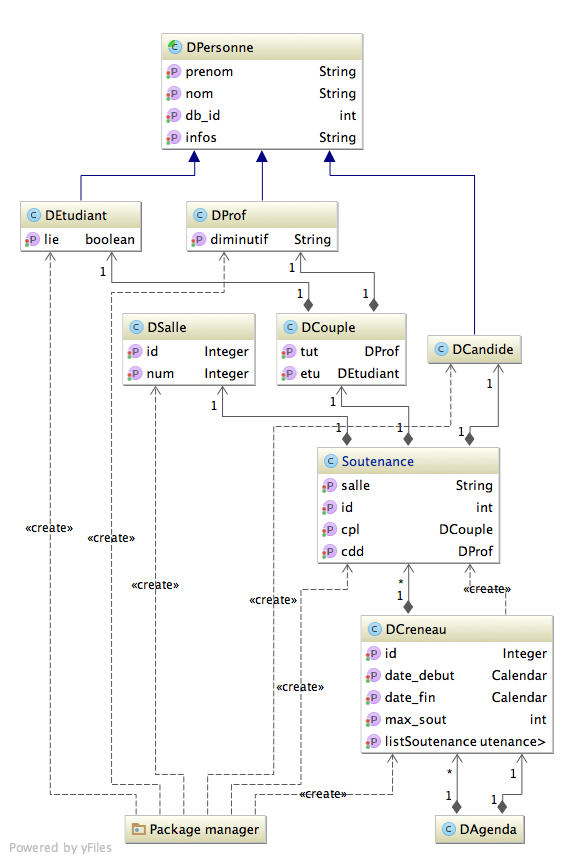
\includegraphics[scale=.5]{uml_don.png}	
				\centering
			\end{figure}

			\paragraph*{}
			Ce schéma montre bien l’enchaînement des objets. On commence par les personnes et on finit par les agendas. On remarque également que le paquet \textit{manager} crée la totalité des objets. Cela vient du fait que les classes de manager instancient ces objets à partir de la base de données.

		\subsection{UML de la vue}

			\begin{figure}[h!]
				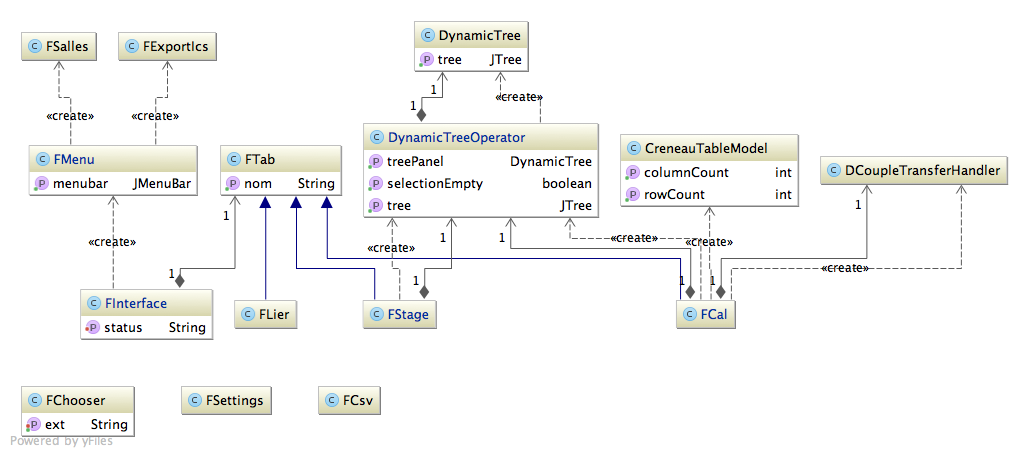
\includegraphics[scale=.5]{uml_fen.png}
				\centering
			\end{figure}

			\paragraph*{}
			Dans ce graphe, on remarque bien que la fenêtre principale (\textit{FInterface}) est composée d’onglets (\textit{FTab}). On remarque également la présence de trois objets hérités de \textit{FTab}, ces derniers constituent les trois onglets de l'application.

	\section{Base de données}

		La base de données est a été conçue à partir du schéma UML du modèle montré précédemment. Elle ne concerne que les données et non la vue ou le contrôleur.

\chapter*{Conclusion}

Nous espérons que nos explications ont été assez claires sur la modélisation de l'application et le rôle de chaque classe. 
Ce projet étant à la fois prometteur et inachevé, il serait intéressant que l'application soit reprise par un futur groupe de projet tuteuré.

\end{document}